% =====================================================================
%  Proposal PERURI Chip Hackathon 2026
%  Secure Battery Identity Chip
%  Kompilasi: pdflatex main.tex (dua kali) atau latexmk -pdf main.tex
% =====================================================================
\documentclass[11pt,a4paper]{article}

% ---------- Tata letak & huruf (meniru template Google Docs) ----------
\usepackage[a4paper,margin=2.5cm]{geometry}
\usepackage[T1]{fontenc}
\usepackage[utf8]{inputenc}
\usepackage[scaled=0.95]{helvet}
\renewcommand{\familydefault}{\sfdefault}
\usepackage{microtype}
\usepackage{amsmath}
\setlength{\parindent}{0pt}
\setlength{\parskip}{4pt}
\linespread{1.08}

\usepackage[table]{xcolor}
\usepackage{graphicx}
\usepackage{tabularx}
\usepackage{array}
\usepackage{enumitem}
\usepackage{titlesec}
\usepackage{caption}
\usepackage{float}
\usepackage{tcolorbox}
\usepackage{pifont}
\newcommand{\cmark}{\textcolor{okline}{\ding{51}}}
\newcommand{\xmark}{\textcolor{badline}{\ding{55}}}
\newcommand{\pmark}{\textcolor{subtle}{\ding{108}}}
\usepackage{fancyhdr}
\usepackage{tikz}
\usetikzlibrary{positioning,arrows.meta,fit,backgrounds,calc}
\usepackage[hidelinks]{hyperref}
\hypersetup{
  pdftitle={Secure Battery Identity Chip},
  pdfauthor={Guntur Sulistyo, Dimas Eryan Ahnaf Fahrezi, Muhammad Muqtada Alhaddad (Universitas Gadjah Mada)},
  pdfsubject={Proposal Hackathon Chip 2026, IC Chip Design \& FPGA Implementation},
}

% ---------- Warna ----------
\definecolor{hdrgreen}{HTML}{E6EFC5}   % header tabel seperti template
\definecolor{subtle}{HTML}{6B7280}
\definecolor{todo}{HTML}{DC2626}
\definecolor{secfill}{HTML}{EEF2FF}
\definecolor{secline}{HTML}{4338CA}
\definecolor{okfill}{HTML}{F0FDF4}
\definecolor{okline}{HTML}{16A34A}
\definecolor{badfill}{HTML}{FEF2F2}
\definecolor{badline}{HTML}{DC2626}
\definecolor{ink}{HTML}{0F172A}

% ---------- Judul bagian ----------
\titleformat{\section}{\fontsize{19}{23}\selectfont\raggedright}{\thesection.}{0.4em}{}
\titleformat{\subsection}{\fontsize{15}{19}\selectfont\raggedright}{\thesubsection}{0.5em}{}
\titleformat{name=\section,numberless}{\fontsize{19}{23}\selectfont\raggedright}{}{0em}{}
\titlespacing*{\section}{0pt}{12pt}{4pt}
\titlespacing*{\subsection}{0pt}{9pt}{3pt}

\newcommand{\field}[1]{\textbf{#1}\par\nobreak}
\newcommand{\todo}[1]{\textcolor{todo}{\textbf{[#1]}}}
\newcommand{\hdr}[1]{\cellcolor{hdrgreen}\textbf{#1}}

\setlist[itemize]{leftmargin=1.4em,itemsep=2pt,topsep=2pt}
\setlist[enumerate]{leftmargin=1.6em,itemsep=2pt,topsep=2pt}
\captionsetup{font=small,labelfont=bf,labelsep=period}
\renewcommand{\figurename}{Gambar}
\renewcommand{\tablename}{Tabel}
\renewcommand{\refname}{}
\renewcommand{\arraystretch}{1.3}

\pagestyle{fancy}
\fancyhf{}
\renewcommand{\headrulewidth}{0pt}
\fancyfoot[C]{\footnotesize\color{subtle}Hackathon CHIP 2026 --- Secure Battery Identity Chip \quad|\quad \thepage}

% =====================================================================
\begin{document}

% =====================================================================
%  COVER (tidak dihitung dalam batas 6 halaman)
% =====================================================================
\begin{titlepage}
\thispagestyle{empty}
\definecolor{coverdark}{HTML}{3F4A1A}
\definecolor{coveraccent}{HTML}{6B7F24}
\definecolor{ink}{HTML}{0F172A}
\definecolor{motif}{HTML}{C5D48A}
\begin{tikzpicture}[remember picture, overlay]
  % --- Pita kiri
  \fill[coverdark] (current page.north west) rectangle ([xshift=9mm]current page.south west);
  \fill[hdrgreen] ([xshift=9mm]current page.north west) rectangle ([xshift=10.5mm]current page.south west);

  % --- Motif chip + sidik jari (PUF), kanan bawah, sebagian keluar halaman
  \coordinate (c) at ([xshift=-36mm, yshift=86mm]current page.south east);
  \begin{scope}[shift={(c)}]
    % badan chip
    \draw[motif, line width=1.1pt, rounded corners=6mm] (-38mm,-38mm) rectangle (38mm,38mm);
    \draw[motif!70, line width=0.6pt, rounded corners=4mm] (-33mm,-33mm) rectangle (33mm,33mm);
    % pin
    \foreach \p in {-27,-18,-9,0,9,18,27} {
      \draw[motif, line width=1.6pt, line cap=round] (\p mm,38mm) -- (\p mm,46mm);
      \draw[motif, line width=1.6pt, line cap=round] (\p mm,-38mm) -- (\p mm,-46mm);
      \draw[motif, line width=1.6pt, line cap=round] (38mm,\p mm) -- (46mm,\p mm);
      \draw[motif, line width=1.6pt, line cap=round] (-38mm,\p mm) -- (-46mm,\p mm);
    }
    % sidik jari: busur konsentris yang terputus secara acak (deterministik)
    \pgfmathsetseed{2026}
    \foreach \r in {3,6,...,27} {
      \foreach \k in {0,1,2,3} {
        \pgfmathsetmacro{\st}{\k*90 + \r*11 + rnd*20}
        \pgfmathsetmacro{\ln}{52 + rnd*26}
        \draw[coveraccent!70, line width=0.9pt, line cap=round]
          ([shift={(\st:\r mm)}]0,0) arc[start angle=\st, delta angle=\ln, radius=\r mm];
      }
    }
    \fill[coveraccent] (0,0) circle (1.2mm);
  \end{scope}

  % --- Garis footer
  \draw[subtle!40, line width=0.4pt]
    ([xshift=25mm, yshift=24mm]current page.south west) -- ([xshift=-25mm, yshift=24mm]current page.south east);
  \node[anchor=north west, font=\footnotesize, text=subtle, inner sep=0]
    at ([xshift=25mm, yshift=20mm]current page.south west) {Universitas Gadjah Mada};
  \node[anchor=north east, font=\footnotesize, text=subtle, inner sep=0]
    at ([xshift=-25mm, yshift=20mm]current page.south east) {Yogyakarta, Oktober 2026};
\end{tikzpicture}

\vspace*{0.6cm}
{\footnotesize\bfseries\color{coveraccent} PROPOSAL PESERTA \quad\textcolor{subtle!60}{|}\quad \textcolor{subtle}{HACKATHON CHIP 2026}\par}
\vspace{3pt}
{\footnotesize\color{subtle} Kategori: IC Chip Design \& FPGA Implementation \,\textperiodcentered\, Topik 1: Secure Identity \& Security Element Chip\par}

\vspace{2.6cm}
{\fontsize{46}{50}\selectfont\bfseries\color{ink} Secure Battery\\[2pt] Identity Chip\par}
\vspace{14pt}
{\color{coveraccent}\rule{2.4cm}{3pt}\par}
\vspace{14pt}
\begin{minipage}{0.86\linewidth}
{\fontsize{15}{20}\selectfont\color{ink!80}\raggedright\hyphenpenalty=10000 Chip keamanan yang membuktikan keaslian baterai di stasiun tukar baterai kendaraan listrik, dengan kunci dari sidik jari silikon (PUF) yang tidak disimpan di chip\par}
\end{minipage}


\vfill
\newcommand{\role}[1]{{\scriptsize\bfseries\color{subtle}#1}}
\newcommand{\person}[2]{{\small\color{ink}#1}\newline{\footnotesize\color{ink!70}Universitas Gadjah Mada}\newline{\footnotesize\color{ink!70}#2}}
\begin{minipage}{0.68\linewidth}
\renewcommand{\arraystretch}{1.2}
\begin{tabular}{@{}>{\raggedright\arraybackslash}p{2.9cm}>{\raggedright\arraybackslash}p{7.6cm}@{}}
\role{NAMA TIM} & {\small\bfseries\color{ink}-NaS} \\[8pt]
\role{KETUA} & \person{Guntur Sulistyo}{guntursulistyo@mail.ugm.ac.id} \\[8pt]
\role{ANGGOTA} & \person{Dimas Eryan Ahnaf Fahrezi}{dimaseryanahnaffahrezi@mail.ugm.ac.id} \\[8pt]
& \person{Muhammad Muqtada Alhaddad}{muhammadmuqtadaalhaddad@mail.ugm.ac.id} \\[8pt]
\role{DOSEN PEMBIMBING} & {\small\color{ink}Ir. Agus Bejo, S.T., M.Eng., D.Eng., IPM}\newline{\footnotesize\color{ink!70}Universitas Gadjah Mada} \\
\end{tabular}
\end{minipage}
\vspace*{1.4cm}
\end{titlepage}

\setcounter{page}{1}

% =====================================================================
\section{Executive Summary}

Setiap hari, pengendara motor listrik menukar baterai kosong dengan baterai penuh di stasiun penukaran baterai (SPBKLU). Baterai tersebut merupakan aset bersama yang berpindah dari satu pengendara ke pengendara lain dan dapat melewati beberapa operator dengan sistem yang berbeda. Saat menerima sebuah baterai, stasiun hanya dapat membaca data yang dilaporkan baterai itu sendiri sehingga keaslian dan catatan pemakaiannya tidak dapat dibuktikan. Baterai palsu atau bekas yang dirakit ulang tanpa standar dapat lolos ke jaringan dan berisiko memicu kebakaran. Jumlah siklus pemakaian juga dapat diubah agar baterai tua tampak baru, seperti odometer mobil bekas yang diputar mundur. Kedua celah ini makin luas seiring bertambahnya motor listrik, yang pada akhir 2024 telah mencapai sekitar 168 ribu unit~\cite{ruptl}.

Kami mengusulkan Secure Battery Identity Chip, chip keamanan kecil yang ditanam di dalam setiap baterai. Kami merancang chip ini untuk membaca ``sidik jari'' alami dari variasi fabrikasi silikonnya dan menurunkan kunci dari sidik jari tersebut setiap kali dibutuhkan. Kunci tidak pernah disimpan di dalam chip, sehingga tidak ada kunci di memori chip yang dapat dibaca atau disalin. Saat baterai masuk, basis data identitas mengirim angka acak sekali pakai (\emph{nonce}) yang hanya dapat dijawab oleh chip asli (Gambar~\ref{fig:konsep}). Catatan pemakaian berasal dari pengukuran stasiun saat mengisi daya dan disimpan di basis data identitas yang dikelola lembaga penjamin keaslian. Jika chip mendeteksi pembongkaran atau gangguan listrik, chip berhenti menjawab dan basis data memblokir identitasnya.

\begin{figure}[H]
\centering
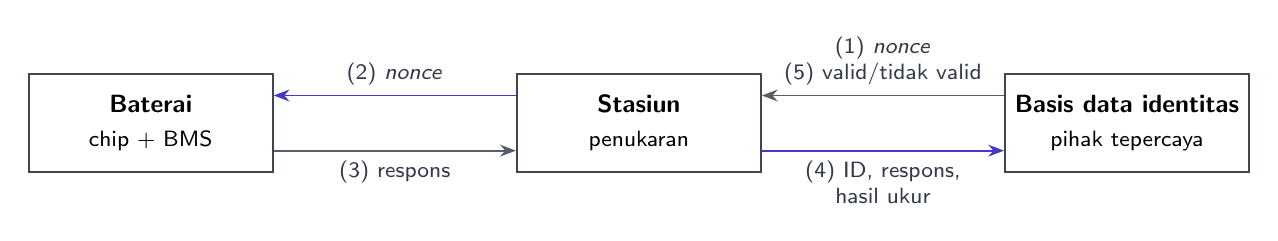
\begin{tikzpicture}[
  font=\sffamily\small,
  actor/.style={draw=ink!80, line width=0.7pt, align=center, minimum width=3.1cm, minimum height=1.25cm, fill=white},
  flow/.style={-{Stealth[length=2mm]}, line width=0.7pt, draw=secline},
  back/.style={-{Stealth[length=2mm]}, line width=0.7pt, draw=ink!70},
  lbl/.style={font=\sffamily\footnotesize, text=ink!85, align=center},
  role/.style={font=\sffamily\footnotesize\itshape, text=subtle, align=center, text width=3.4cm}
]
  \node[actor] (pack) at (0,0)    {\textbf{Baterai}\\[1pt]\footnotesize chip + BMS};
  \node[actor] (st)   at (6.2,0)  {\textbf{Stasiun}\\[1pt]\footnotesize penukaran};
  \node[actor] (reg)  at (12.4,0) {\textbf{Basis data identitas}\\[1pt]\footnotesize pihak tepercaya};

  \draw[back] ([yshift=3.5mm]reg.west) -- node[lbl, above]{(1) \emph{nonce}\\(5) valid/tidak valid} ([yshift=3.5mm]st.east);
  \draw[flow] ([yshift=3.5mm]st.west) -- node[lbl, above]{(2) \emph{nonce}} ([yshift=3.5mm]pack.east);
  \draw[back] ([yshift=-3.5mm]pack.east) -- node[lbl, below]{(3) respons} ([yshift=-3.5mm]st.west);
  \draw[flow] ([yshift=-3.5mm]st.east) -- node[lbl, below]{(4) ID, respons,\\hasil ukur} ([yshift=-3.5mm]reg.west);

\end{tikzpicture}
\caption{Alur verifikasi baterai di stasiun penukaran.}
\label{fig:konsep}
\end{figure}

Riwayat tersebut hanya bermakna apabila identitas baterai tidak dapat dipalsukan. Karena itu, identitas diwujudkan sebagai chip di dalam baterai, satu-satunya komponen yang ikut berpindah bersama baterai dan dapat dirancang untuk menahan serangan fisik.

\begin{center}
\small
\renewcommand{\arraystretch}{1.12}
\begin{tabularx}{\linewidth}{|>{\raggedright\arraybackslash}p{3.1cm}|X|}
\hline
\hdr{Chip yang dirancang} & \emph{Secure element} tanpa memori non-volatil untuk kunci dan data, berisi \emph{Ring-Oscillator PUF} dengan \emph{fuzzy extractor}, HMAC-SHA-256, FSM \emph{challenge--response}, dan monitor \emph{tamper}. Target ASIC SKY130. \\ \hline
\hdr{Target pengguna} & Operator stasiun dan penyedia sewa baterai (pemeriksa), produsen baterai dan BMS (pemasang chip), serta lembaga penjamin keaslian (pengelola basis data identitas). Adopsi dapat didorong melalui standar identitas baterai. \\ \hline
\hdr{Dampak} & Baterai yang tidak dikenal ditolak sebelum diserahkan (keselamatan). Harga jual kembali dan garansi ditentukan dari riwayat yang tepercaya (ekonomi). Akar kepercayaan dirancang di dalam negeri (kemandirian). \\ \hline
\hdr{Status prototipe} & SHA-256, HMAC, FSM, dan \emph{zeroize} lolos simulasi Verilator. PUF masih model LFSR. Uji di DE10-Nano dan PUF fisik direncanakan. \\ \hline
\end{tabularx}
\end{center}

Kebaruan usulan ini terletak pada pembagian peran yang tegas. Chip membuktikan identitas, stasiun mengukur, dan basis data mengingat. Dengan pembagian ini, chip tetap kecil, tanpa memori non-volatil untuk kunci dan data, dan dapat diverifikasi oleh operator mana pun yang terhubung ke basis data identitas.


% =====================================================================
\section{Problem Statement}

\subsection{Latar Belakang}

Percepatan kendaraan bermotor listrik berbasis baterai diatur melalui Perpres No.~55 Tahun 2019 dan perubahannya, Perpres No.~79 Tahun 2023~\cite{perpres55,perpres79}. Hingga Desember 2024, jumlah kendaraan listrik roda dua telah mencapai sekitar 168 ribu unit, lebih dari dua kali jumlah roda empat~\cite{ruptl}. Untuk segmen ini dikembangkan Stasiun Penukaran Baterai Kendaraan Listrik Umum (SPBKLU), yang dalam RUPTL PLN 2025--2034 diintegrasikan ke dalam platform layanan kendaraan listrik PLN~\cite{ruptl}. Skalanya akan terus membesar karena RUKN menargetkan penetrasi sepeda motor listrik sebanyak 2,9--3,8 juta unit pada 2030 dan 5,5--5,7 juta unit pada 2035~\cite{rukn}. Pada model tukar baterai, pengendara hanya menyewa baterai milik operator atau penyedia sewa. Setelah diisi ulang di stasiun, baterai yang sama diserahkan kepada pengendara lain, sehingga sebagian besar masa pakainya berlangsung di luar pengawasan pemiliknya. Badan usaha SPBKLU cukup memiliki NIB dan nomor identitas SPBKLU tanpa izin usaha penyediaan tenaga listrik~\cite{rukn}, sehingga operator dengan sistem yang berbeda dapat terus bertambah. Di tingkat global, Regulasi Baterai Uni Eropa 2023/1542 mewajibkan paspor baterai digital, termasuk untuk baterai kendaraan ringan~\cite{eubat}. Identitas baterai yang dapat diverifikasi mulai menjadi kebutuhan yang diatur.

\subsection{Tiga Masalah Inti}

Seperti dokumen berharga, baterai tukar terus berpindah tangan. Karena itu, keaslian dan riwayatnya perlu dibuktikan secara elektronik di setiap stasiun yang menerimanya. Tiga masalah muncul dari kebutuhan tersebut.

\begin{enumerate}[label=\textbf{P\arabic*.}, leftmargin=2.2em]
  \item \textbf{Keaslian baterai tidak dapat dibuktikan secara independen.} Nomor seri, label, dan kode QR mudah disalin, sedangkan autentikasi milik operator hanya berlaku di jaringannya sendiri. Pihak yang mencari keuntungan dapat menyerahkan baterai palsu di stasiun dan membawa pulang baterai asli. Operator kehilangan aset, sedangkan pengendara berikutnya menerima baterai dengan sel yang berisiko mengalami \emph{thermal runaway}.
  \item \textbf{Riwayat baterai hanya bersumber dari data yang dilaporkan baterai itu sendiri.} Jumlah siklus dan kondisi kesehatan dilaporkan oleh BMS (\emph{Battery Management System}), papan pengendali di dalam \emph{pack} baterai, yaitu satu unit berisi sel, BMS, dan casing. BMS dapat diprogram ulang untuk memalsukan data tersebut. Padahal, harga jual kembali, klaim garansi, dan keputusan keselamatan ditentukan dari data itu.
  \item \textbf{Kepercayaan tidak berlaku lintas operator.} Operator yang bersaing cenderung tidak mempercayai basis data milik pesaingnya. Ketika baterai mulai distandarkan antaroperator, baterai yang ditolak di satu jaringan dapat beredar di jaringan lain. Pembeli baterai bekas, pihak daur ulang, dan penjamin garansi juga tidak memiliki sumber netral untuk memeriksa riwayatnya.
\end{enumerate}

\subsection{Alasan Diperlukannya Chip}

Identitas baterai tidak dapat diserahkan kepada perangkat lunak. Pemalsu memegang baterai tanpa batas waktu, sehingga firmware dapat diprogram ulang dan kunci di memori flash dapat diekstrak melalui \emph{probing} atau \emph{fault injection}~\cite{barel}. Satu kunci asli yang bocor kemudian dapat disalin ke banyak baterai palsu. Karena itu, akar kepercayaan harus berada di silikon dengan tiga syarat, yaitu kunci tidak tersimpan di chip~\cite{suh,maes}, kriptografi terisolasi dari firmware, dan chip mampu merespons serangan fisik secara mandiri. Chip asli yang dipindahkan ke \emph{pack} baterai palsu tetap dapat menjawab dengan benar. Celah ini dipersempit di tingkat sistem dengan mencocokkan hasil ukur sel terhadap riwayat identitasnya.

\subsection{Kesenjangan Solusi yang Tersedia}
\newcommand{\sbg}{{\footnotesize\color{subtle}sebagian}}

\begin{center}
\small
\renewcommand{\arraystretch}{1.15}
\renewcommand{\tabularxcolumn}[1]{m{#1}}
\begin{tabularx}{\linewidth}{|>{\raggedright\arraybackslash}X|*{6}{>{\centering\arraybackslash\hyphenpenalty=10000\exhyphenpenalty=10000}m{1.5cm}|}}
\hline
\hdr{Pendekatan} & \hdr{Sulit dikloning} & \hdr{Tahan serangan fisik} & \hdr{Tanpa kunci di chip} & \hdr{Desain dapat diperiksa} & \hdr{Enrolment pihak tepercaya} & \hdr{Riwayat lintas operator} \\ \hline
Label atau kode QR & \xmark & \xmark & -- & -- & \sbg & \sbg \\ \hline
Kunci di firmware BMS & \xmark & \xmark & \xmark & \sbg & \xmark & \xmark \\ \hline
IC dengan kunci tersimpan\newline{\footnotesize\color{subtle}contoh: TI bq, OPTIGA} & \cmark & \cmark & \xmark & \xmark & \sbg & \xmark \\ \hline
IC berbasis PUF\newline{\footnotesize\color{subtle}contoh: DS28E38} & \cmark & \cmark & \cmark & \xmark & \cmark & \xmark \\ \hline
\textbf{Usulan}\newline{\footnotesize\color{subtle}target desain} & \cmark & \sbg & \cmark & \cmark & \cmark & \cmark \\ \hline
\end{tabularx}
\end{center}

IC komersial sudah tahan kloning dan serangan fisik, baik yang menyimpan kunci di memori~\cite{bq26100} maupun yang menurunkan kunci dari PUF seperti DS28E38~\cite{ds28e38}. Namun, keduanya berdesain tertutup sehingga pihak tepercaya tidak dapat memeriksa cara kunci dibangkitkan. Pembeda usulan ini adalah RTL terbuka yang dapat diperiksa dan integrasi dengan basis data identitas lintas operator.

\subsection{Rumusan Masalah dan Kebutuhan Desain}

Perancangan diarahkan untuk menjawab satu pertanyaan, yaitu bagaimana membangun \emph{secure element} yang memenuhi lima kebutuhan berikut dengan area cukup kecil untuk ditanam di setiap pack baterai. Semua angka pada tabel berikut adalah target yang akan diukur selama pengembangan.

\begin{center}
\small
\renewcommand{\arraystretch}{1.15}
\begin{tabularx}{\linewidth}{|c|>{\raggedright\arraybackslash}p{2.7cm}|>{\raggedright\arraybackslash}X|>{\raggedright\arraybackslash}p{4.0cm}|}
\hline
\hdr{ID} & \hdr{Kebutuhan} & \hdr{Target} & \hdr{Cara mengukur} \\ \hline
R1 & Sulit dikloning & Kunci dari PUF, tidak disimpan. Kunci tetap sama pada $\geq$1.000 kali pembacaan di suhu ruang dan berbeda antar-chip (\emph{Hamming distance} $\approx$50\%) & Bandingkan kunci tiap pembacaan, antar-lokasi RO, dan antar-board \\ \hline
R2 & Tahan \emph{replay} & Respons lama selalu ditolak. Respons selesai $<$50 ms & Uji \emph{replay} dan hitung \emph{clock cycle} \\ \hline
R3 & Riwayat tepercaya & Riwayat berasal dari pengukuran stasiun. Perubahan sel yang janggal ditandai & Skenario demo dengan basis data emulasi \\ \hline
R4 & \emph{Fail-secure} & \emph{Glitch} clock atau casing terbuka $\rightarrow$ kunci dihapus dan chip terkunci & \emph{Glitch} melalui PLL dan pin \emph{tamper} \\ \hline
R5 & Kecil, siap ASIC & Tanpa NVM untuk data, tanpa DSP, $<$15\% ALM Cyclone~V & Sintesis Quartus dan Yosys \\ \hline
\end{tabularx}
\end{center}

% =====================================================================
\section{Proposed Chip}

\subsection{Fungsi Utama}

Chip ini memiliki satu fungsi inti, yaitu membuktikan identitas \emph{pack} baterai kepada basis data identitas melalui stasiun, tanpa menyimpan kunci di dalam chip. Variasi fabrikasi membuat setiap chip memiliki ``sidik jari'' silikon yang unik. Rangkaian \emph{Ring-Oscillator PUF} (RO-PUF) membaca sidik jari ini setiap kali dibutuhkan. Chip kemudian menurunkan kunci darinya, menghitung respons atas \emph{nonce} dari basis data identitas, dan langsung menghapus kunci.

\subsection{Arsitektur dan Alur Data}

\begin{figure}[H]
\centering
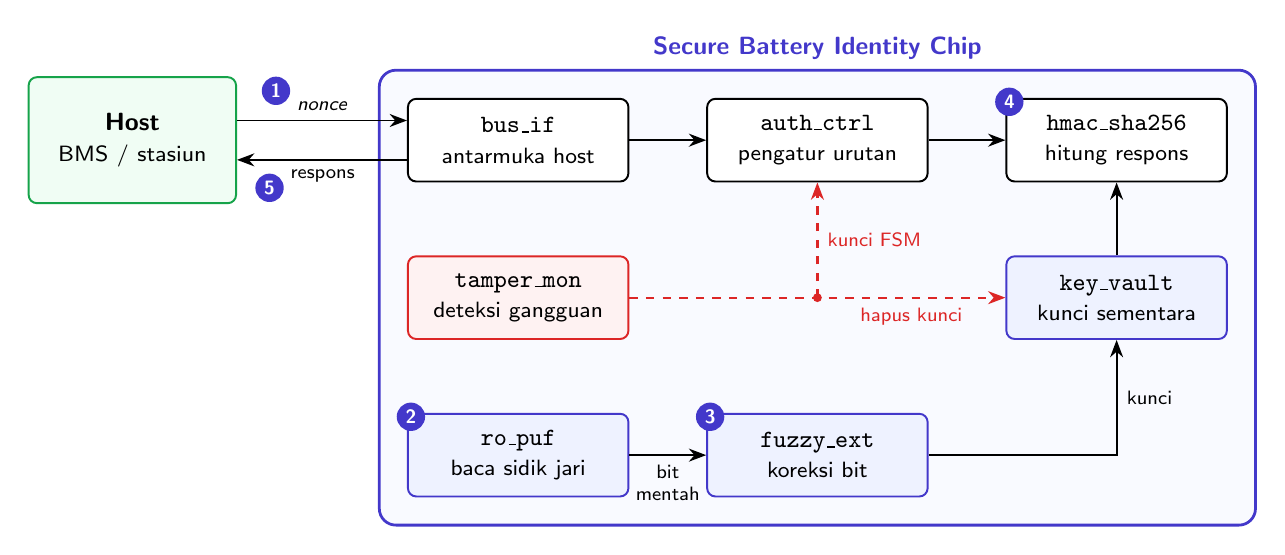
\begin{tikzpicture}[
  font=\sffamily\small,
  blk/.style={draw, rounded corners=3pt, align=center, minimum height=1.05cm, minimum width=2.8cm, fill=white, line width=0.7pt},
  key/.style={blk, fill=secfill, draw=secline},
  mon/.style={blk, fill=badfill, draw=badline},
  host/.style={blk, fill=okfill, draw=okline, minimum width=2.6cm, text width=2.4cm},
  arr/.style={-{Stealth[length=2.2mm]}, line width=0.7pt},
  zer/.style={-{Stealth[length=2.2mm]}, line width=0.8pt, draw=badline, dashed},
  lbl/.style={font=\sffamily\scriptsize, align=center},
  langkah/.style={circle, fill=secline, text=white, font=\sffamily\scriptsize\bfseries, inner sep=1pt, minimum size=3.6mm}
]
  \node[blk] (bus)  at (0,0)     {\texttt{bus\_if}\\\footnotesize antarmuka host};
  \node[blk] (ctrl) at (3.8,0)  {\texttt{auth\_ctrl}\\\footnotesize pengatur urutan};
  \node[blk] (hmac) at (7.6,0)   {\texttt{hmac\_sha256}\\\footnotesize hitung respons};
  \node[mon] (tamp)  at (0,-2)   {\texttt{tamper\_mon}\\\footnotesize deteksi gangguan};
  \node[key] (vault) at (7.6,-2) {\texttt{key\_vault}\\\footnotesize kunci sementara};
  \node[key] (puf) at (0,-4)     {\texttt{ro\_puf}\\\footnotesize baca sidik jari};
  \node[key] (fe)  at (3.8,-4)  {\texttt{fuzzy\_ext}\\\footnotesize koreksi bit};
  \node[host, minimum height=1.6cm] (hps) at (-4.9,0) {\textbf{Host}\\\footnotesize BMS / stasiun};

  \begin{scope}[on background layer]
    \node[draw=secline, line width=1pt, rounded corners=6pt, fill=secfill!35, inner sep=10pt,
          fit=(bus)(ctrl)(hmac)(vault)(fe)(puf)(tamp),
          label={[font=\sffamily\small\bfseries, text=secline]above:Secure Battery Identity Chip}] (chip) {};
  \end{scope}

  % jalur perintah
  \draw[arr] ([yshift=2.5mm]hps.east) -- node[lbl, above, pos=0.4]{\tikz[baseline=-0.6ex]\node[langkah]{1}; \emph{nonce}} ([yshift=2.5mm]bus.west);
  \draw[arr] ([yshift=-2.5mm]bus.west) -- node[lbl, below, pos=0.6]{\tikz[baseline=-0.6ex]\node[langkah]{5}; respons} ([yshift=-2.5mm]hps.east);
  \draw[arr] (bus) -- (ctrl);
  \draw[arr] (ctrl) -- (hmac);
  % jalur kunci
  \draw[arr] (puf) -- node[lbl, below]{bit\\mentah} (fe);
  \draw[arr] (fe.east) -- (7.6,-4) -- node[lbl, right]{kunci} (vault.south);
  \draw[arr] (vault) -- (hmac);
  % jalur pengaman
  \draw[zer] (tamp.east) -- node[lbl, below, text=badline, pos=0.75]{hapus kunci} (vault.west);
  \draw[zer] (3.8,-2) -- node[lbl, right, text=badline]{kunci FSM} (ctrl.south);
  \fill[badline] (3.8,-2) circle (1.6pt);

  % urutan langkah
  \node[langkah] at ([xshift=0.5mm, yshift=-0.5mm]puf.north west) {2};
  \node[langkah] at ([xshift=0.5mm, yshift=-0.5mm]fe.north west) {3};
  \node[langkah] at ([xshift=0.5mm, yshift=-0.5mm]hmac.north west) {4};
\end{tikzpicture}
\caption{Arsitektur chip. Nomor menunjukkan urutan satu autentikasi.}
\label{fig:arsitektur}
\end{figure}

Satu autentikasi berjalan sesuai nomor pada Gambar~\ref{fig:arsitektur}. Host mengirim \emph{nonce} dan \emph{helper data} melalui \texttt{bus\_if} (1). \texttt{ro\_puf} membaca sidik jari silikon (2), lalu \texttt{fuzzy\_ext} mengoreksi bitnya dengan bantuan \emph{helper data} dan menurunkan kunci ke \texttt{key\_vault} (3). \texttt{hmac\_sha256} menghitung respons dari kunci dan \emph{nonce} (4). Kunci kemudian dihapus dan respons dikirim ke host (5). Sepanjang waktu, \texttt{tamper\_mon} memantau clock dan casing. Bila ada gangguan, kunci langsung dihapus dan chip terkunci. Kunci tidak pernah keluar dari chip.

\subsection{Data, Antarmuka, dan Memori}

\begin{center}
\small
\renewcommand{\arraystretch}{1.15}
\begin{tabularx}{\linewidth}{|>{\raggedright\arraybackslash}p{2.2cm}|>{\centering\arraybackslash}p{1.3cm}|>{\centering\arraybackslash}p{1.4cm}|>{\raggedright\arraybackslash}X|>{\raggedright\arraybackslash}p{4.1cm}|}
\hline
\hdr{Data} & \hdr{Ukuran} & \hdr{Sifat} & \hdr{Tempat} & \hdr{Berlaku} \\ \hline
Kunci & 256 bit & Rahasia & Register di dalam chip & Satu autentikasi \\ \hline
\emph{Helper data} & 512 bit & Publik & BMS dan basis data identitas & Tetap sejak enrolment \\ \hline
ID & 64 bit & Publik & Dihitung chip dari \emph{helper data} & Tetap \\ \hline
\emph{Nonce} & 256 bit & Publik & Dibuat basis data identitas & Sekali pakai \\ \hline
Respons & 256 bit & Publik & Dikirim ke basis data melalui stasiun & Sekali pakai \\ \hline
Status \emph{lock} & 1 bit & Publik & Register di dalam chip & Selama chip berdaya \\ \hline
\end{tabularx}
\end{center}

\subsection{Alur Operasi}

\begin{enumerate}
  \item \textbf{Enrolment} --- dilakukan sekali di pabrik baterai di bawah pengawasan lembaga penjamin keaslian. Chip mengirim kuncinya ke HSM dalam keadaan terenkripsi dengan kunci publik HSM yang tertanam di \emph{bitstream} pabrik. Basis data identitas mencatat \emph{helper data}, ID, dan karakteristik awal \emph{pack} baterai. Jalur pengiriman kunci ini hanya ada pada \emph{bitstream} pabrik. Pada ASIC, jalur tersebut ditutup permanen dengan eFuse setelah enrolment.
  \item \textbf{Verifikasi} --- dilakukan pada setiap penukaran baterai. Stasiun meneruskan \emph{nonce} dari basis data identitas ke chip. Chip menjawab dengan respons HMAC$(K, \text{nonce}\,\|\,\text{ID})$. Basis data memeriksa respons tersebut bersama hasil ukur sel, memperbarui riwayat, lalu menjawab \emph{valid} atau \emph{tidak valid}. Stasiun tidak pernah memegang kunci.
\end{enumerate}

Chip yang terkunci tetap mendapat daya dari sel, sehingga statusnya terbaca oleh stasiun berikutnya dan basis data memblokir ID tersebut.

% =====================================================================
\section{Technical Design}

\subsection{Rincian Modul RTL}

\begin{center}
\footnotesize
\renewcommand{\arraystretch}{1.15}
\begin{tabularx}{\linewidth}{|>{\raggedright\arraybackslash}p{2.0cm}|>{\raggedright\arraybackslash}p{3.9cm}|X|}
\hline
\hdr{Modul} & \hdr{Tugas} & \hdr{Cara kerja} \\ \hline
\texttt{bus\_if} & Antarmuka ke host & Register AXI-Lite (FPGA) atau I\textsuperscript{2}C (ASIC). Kunci tidak dapat dibaca melalui bus. \\ \hline
\texttt{auth\_ctrl} & Mengatur urutan perintah & FSM \texttt{GET\_ID}, \texttt{AUTH}, dan \texttt{STATUS}. Membatasi laju \texttt{AUTH} dan menolak perintah saat \emph{lock}. \\ \hline
\texttt{ro\_puf} & Membaca sidik jari silikon & \emph{Ring oscillator} dibandingkan berpasangan. Model RTL saat ini LFSR deterministik untuk simulasi. \\ \hline
\texttt{fuzzy\_ext} & Membuat bit PUF stabil & \emph{Majority voting} dan kode repetisi untuk membuang bit yang berubah-ubah. Bit stabil di-\emph{hash} SHA-256 menjadi kunci 256 bit (target entropi $\geq$128 bit). \\ \hline
\texttt{key\_vault} & Menyimpan kunci sementara & Menyimpan kunci hanya selama respons dihitung, lalu menghapusnya. Isinya tidak dapat dibaca dari luar chip. \\ \hline
\texttt{hmac\_sha256} & Menghitung respons & Inti SHA-256 iteratif dan wrapper HMAC-SHA-256; kunci diberikan oleh blok PUF atau model perilakunya. \\ \hline
\texttt{tamper\_mon} & Mendeteksi gangguan & Memantau clock dan sakelar casing, lalu memicu hapus kunci dan \emph{lock}. \\ \hline
\end{tabularx}
\end{center}

\subsection{Implementasi dan Estimasi Kinerja}

\textbf{Target prototipe FPGA.} Desain ditujukan untuk bagian FPGA Cyclone~V pada DE10-Nano. Prosesor ARM (HPS) pada board yang sama berperan sebagai BMS, stasiun, dan basis data identitas yang diemulasikan dengan Python. Karena antarmukanya sederhana dan tanpa NVM, desain ini juga dapat dipasang sebagai blok tambahan pada baseline chip penyelenggara~\cite{peruri}. Kompilasi awal di Quartus Prime sudah berhasil hingga tahap Assembler dengan Fmax 86,85~MHz (\emph{constraint} clock belum final).

\begin{table}[!b]
\centering
\small
\renewcommand{\arraystretch}{1.15}
\begin{tabular}{|l|c|c|c|}
\hline
\hdr{Komponen} & \hdr{Estimasi} & \hdr{Kompilasi awal} & \hdr{Kapasitas} \\ \hline
Logika (ALM) & $\approx$4.000--6.000 & 2.386 (5,7\%) & 41.910 \\ \hline
Register & $\approx$3.000--5.000 & 4.341 (2,6\%) & 166.036 \\ \hline
Blok RAM (M10K) & 0--2 & 0 & 553 \\ \hline
DSP & 0 & 0 & 112 \\ \hline
\end{tabular}
\caption{Sumber daya FPGA DE10-Nano. Kompilasi awal belum memuat seluruh blok IP.}
\end{table}

\textbf{Kecepatan.} Satu perhitungan HMAC membutuhkan sekitar 280 siklus clock, atau 5,6\,$\mu$s pada 50~MHz. Bagian terlama adalah pembacaan ulang PUF, dengan target total respons di bawah 50~ms.

\textbf{Daya dan versi ASIC.} Di luar autentikasi, hanya \texttt{tamper\_mon} yang aktif dengan clock lambat. Versi ASIC ditargetkan pada proses SkyWater SKY130 (130~nm) dengan area di bawah 0,5~mm\textsuperscript{2} dan daya siaga di bawah 1~mW, jauh lebih kecil daripada pengosongan alami baterai. Daya dan area akan diestimasi dengan Quartus Power Analyzer, Yosys, dan OpenROAD.

\subsection{Strategi Verifikasi}

\begin{itemize}
  \item \textbf{Verifikasi RTL yang telah dijalankan} --- \emph{Testbench} C++ dengan Verilator membandingkan SHA-256 dengan vektor pesan kosong, \texttt{abc}, dan \texttt{hello}, serta HMAC dengan RFC 4231 kasus 1 dan model Python. Uji integrasi melalui AXI meloloskan tag cocok, menolak tag salah, dan menjalankan \emph{zeroize}. PUF masih model LFSR, sehingga belum ada hasil PUF fisik yang diklaim.
  \item \textbf{Verifikasi lanjutan} --- Di DE10-Nano akan diuji karakterisasi PUF fisik (R1), uji \emph{replay} (R2), skenario basis data (R3), serta \emph{glitch} dan \emph{tamper} (R4), dengan statistik dan latensi dari pengukuran aktual.
\end{itemize}

% =====================================================================
\section{Security Design}

\subsection{Model Ancaman}

\begin{center}
\footnotesize
\renewcommand{\arraystretch}{1.2}
\begin{tabularx}{\linewidth}{|>{\raggedright\arraybackslash}p{2.3cm}|>{\raggedright\arraybackslash}X|>{\raggedright\arraybackslash}p{6.6cm}|}
\hline
\hdr{Pelaku} & \hdr{Serangan} & \hdr{Cara menangkal} \\ \hline
Pemalsu baterai & Menyalin chip atau firmware asli & Kunci dari PUF, tidak tersimpan di chip (R1) \\ \hline
Pemalsu baterai & Memindahkan chip asli ke baterai palsu & Hasil ukur sel dicocokkan dengan riwayat ID (R3) \\ \hline
Penyadap & Mengirim ulang respons lama & Setiap \emph{nonce} hanya berlaku sekali (R2) \\ \hline
Bengkel nakal & Mengubah jumlah siklus di BMS & Riwayat dari pengukuran stasiun, bukan BMS (R3) \\ \hline
Stasiun curang & Mengirim hasil ukur palsu & Dicocokkan dengan data stasiun lain (R3) \\ \hline
Penyerang fisik & Mengganggu clock atau membuka casing & Kunci dihapus dan chip terkunci (R4) \\ \hline
Penyerang fisik & Mematikan daya untuk membuka kunci & Basis data memblokir ID yang pernah terkunci \\ \hline
Penyerang fisik & Mengambil kunci melalui \texttt{ENROLL} & \texttt{ENROLL} tidak ada di chip lapangan \\ \hline
Penyerang fisik & Mengubah \emph{helper data} & Kunci menjadi salah sehingga respons ditolak \\ \hline
\end{tabularx}
\end{center}

\subsection{Prinsip \emph{Security-by-Design}}

\begin{itemize}
  \item \textbf{Tidak ada kunci di lapangan.} Stasiun dan BMS tidak pernah memegang kunci. Chip hanya membentuk kunci selama satu autentikasi. Salinannya hanya disimpan di HSM pihak tepercaya.
  \item \textbf{Gangguan berarti terkunci.} Bila chip mendeteksi gangguan, kunci langsung dihapus dan chip berhenti menjawab.
  \item \textbf{Basis data yang memutuskan.} Chip hanya membuktikan identitas. Keputusan menerima atau menolak baterai diambil basis data berdasarkan riwayatnya.
\end{itemize}

\subsection{Batasan dan Pengembangan Lanjutan}

\begin{itemize}
  \item \textbf{Belum diuji pada prototipe.} Serangan \emph{side-channel} serta kestabilan PUF terhadap suhu dan penuaan.
  \item \textbf{Ketergantungan pada HSM.} Kunci simetris membuat salinan kunci di HSM menjadi titik rawan tunggal. Versi ASIC direncanakan menggunakan tanda tangan ECC sehingga basis data cukup menyimpan kunci publik dan verifikasi dapat dilakukan tanpa koneksi.
  \item \textbf{Keamanan \emph{bitstream}.} Pada prototipe, \emph{bitstream} FPGA diasumsikan tidak diubah pihak lain. Status \emph{lock} juga hilang bila daya diputus sebelum terbaca stasiun. Versi ASIC direncanakan menyimpan status \emph{lock} pada satu bit eFuse.
  \item \textbf{Rencana cadangan.} Bila PUF belum stabil, demo menggunakan kunci tetap.
\end{itemize}

% =====================================================================
\clearpage
\section*{Daftar Pustaka}
\vspace{-14pt}
\begin{thebibliography}{99}\small
\bibitem{ruptl} PT PLN (Persero), \emph{Rencana Usaha Penyediaan Tenaga Listrik (RUPTL) 2025--2034}, hlm.~II-53--II-54.
\bibitem{perpres55} Peraturan Presiden RI No.~55 Tahun 2019 tentang Percepatan Program Kendaraan Bermotor Listrik Berbasis Baterai untuk Transportasi Jalan.
\bibitem{perpres79} Peraturan Presiden RI No.~79 Tahun 2023 tentang Perubahan atas Perpres No.~55 Tahun 2019.
\bibitem{rukn} Kementerian ESDM, \emph{Rencana Umum Ketenagalistrikan Nasional (RUKN)}, Kepmen ESDM No.~85.K/TL.01/MEM.L/2025, hlm.~51.
\bibitem{eubat} Regulation (EU) 2023/1542 of the European Parliament and of the Council of 12 July 2023 concerning batteries and waste batteries.
\bibitem{barel} H. Bar-El \emph{et al.}, ``The Sorcerer's Apprentice Guide to Fault Attacks,'' \emph{Proceedings of the IEEE}, vol.~94, no.~2, 2006.
\bibitem{suh} G. E. Suh and S. Devadas, ``Physical Unclonable Functions for Device Authentication and Secret Key Generation,'' \emph{Proc. Design Automation Conference (DAC)}, 2007.
\bibitem{maes} R. Maes, \emph{Physically Unclonable Functions: Constructions, Properties and Applications}, Springer, 2013.
\bibitem{bq26100} Texas Instruments, \emph{bq26100: SHA-1/HMAC Based Security and Authentication IC with SDQ Interface}, datasheet.
\bibitem{ds28e38} Analog Devices, \emph{DS28E38: DeepCover Secure ECDSA Authenticator with ChipDNA PUF Protection}, datasheet.
\bibitem{peruri} PERURI, \emph{Peruri Chip Design Datasheet}, chip.peruri.co.id/datasheet.pdf
\end{thebibliography}

% =====================================================================
\clearpage
\section*{Lampiran Teknis}

\begin{itemize}
  \item Repositori proyek (RTL, testbench, model Python, dokumentasi): \url{https://github.com/Grsliy/Heketon-bang}.
  \item Hasil awal model referensi Python (perangkat lunak, kunci tetap): lolos 2 vektor uji SHA-256 FIPS 180-4, 6 vektor uji HMAC-SHA-256 RFC 4231, dan 7 skenario protokol (baterai asli diterima, kloning, \emph{replay}, \emph{helper data} palsu, \emph{tamper}, dan kapasitas tidak wajar ditolak).
  \item Perangkat lunak: Intel Quartus Prime Standard (sintesis, timing, LogicLock, SignalTap), Platform Designer, Verilator, dan Python. Yosys/OpenROAD dengan SkyWater SKY130 PDK merupakan opsi untuk pengembangan ASIC.
  \item Register map, termasuk register tag autentikasi pada alamat 0x80--0x9C dan status \emph{zeroize}, akan dilengkapi pada laporan teknis.
\end{itemize}

Cuplikan berikut berasal dari proyek Quartus Prime Standard untuk Cyclone~V (5CSEBA6U23I7). Kompilasi yang ditampilkan berhasil hingga tahap \emph{Assembler}; laporan mencatat penggunaan sumber daya dan Fmax 86,85~MHz pada clock \texttt{h2f\_user0\_clk}. Constraint timing belum final, sehingga angka ini merupakan hasil awal prototipe dan bukan hasil sign-off. Tampilan Platform Designer memperlihatkan integrasi HPS dan HEKETON melalui lightweight AXI.

\begin{figure}[H]
  \centering
  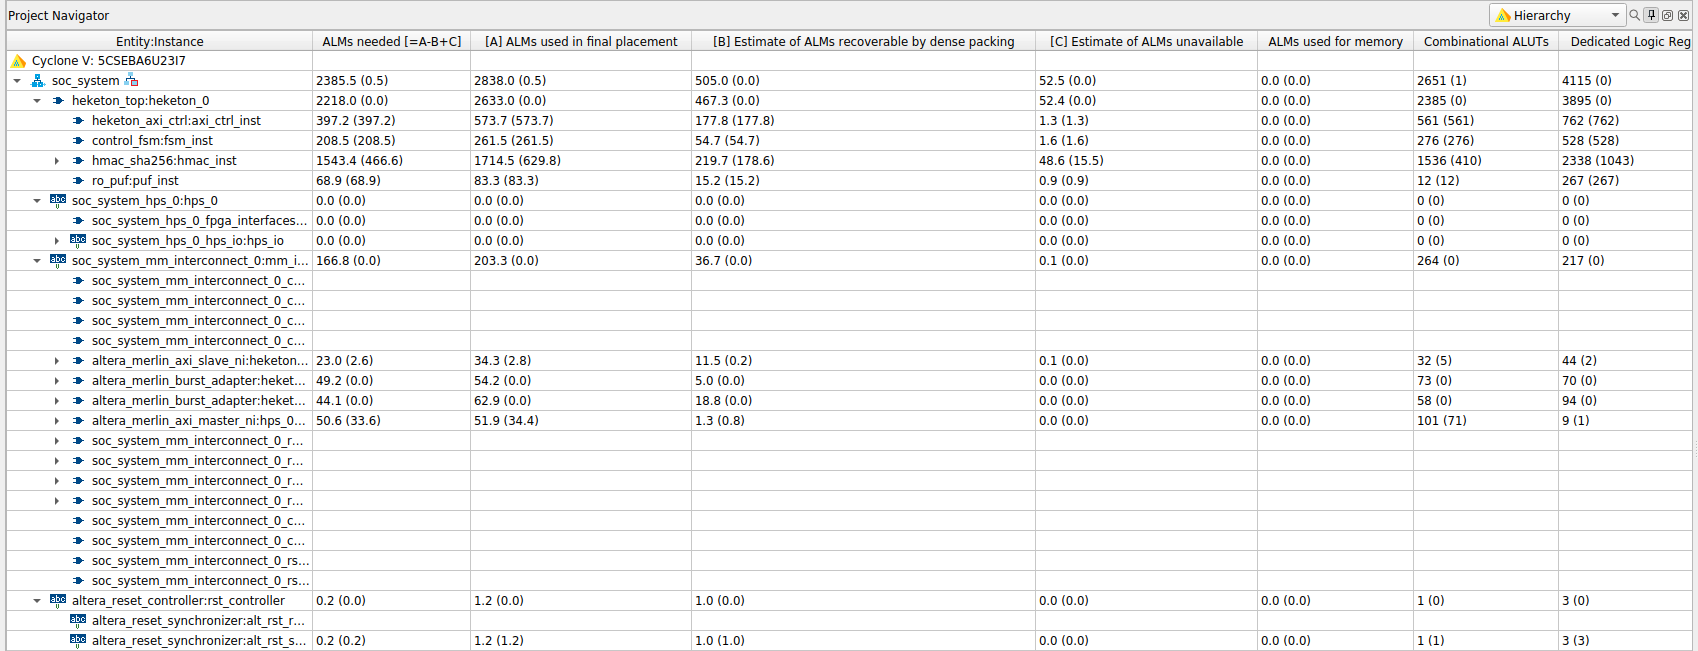
\includegraphics[width=\linewidth,height=0.27\textheight,keepaspectratio]{projectnav.png}
  \caption{Hierarki hasil fitter Quartus dengan estimasi penggunaan ALM per blok RTL.}
\end{figure}

\begin{figure}[H]
  \centering
  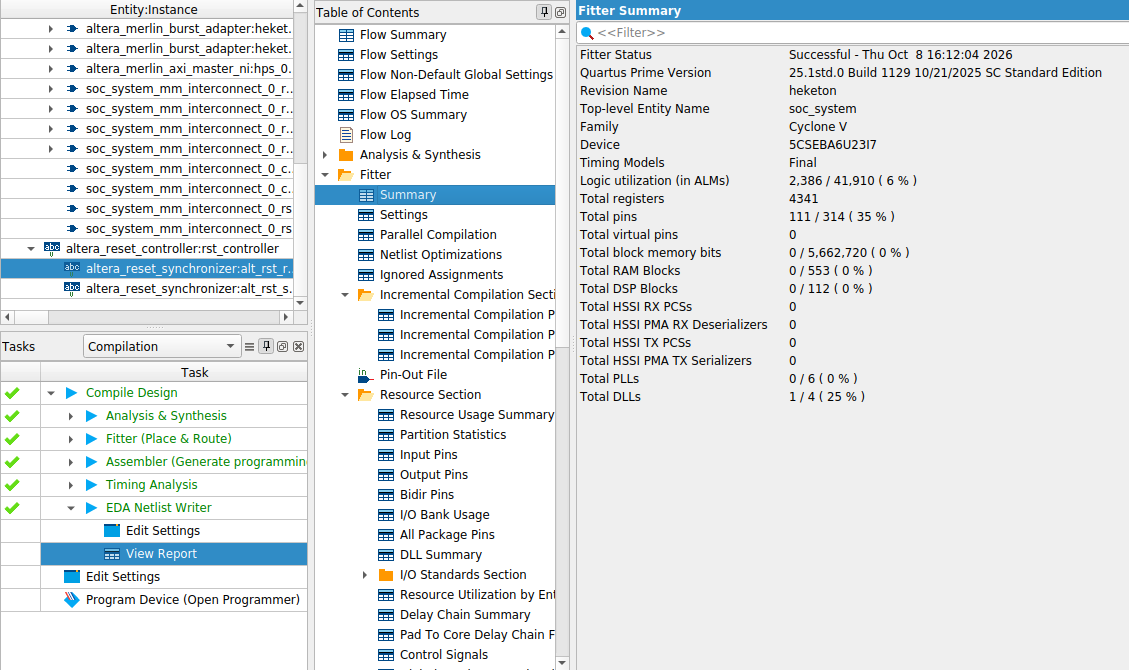
\includegraphics[width=\linewidth,height=0.27\textheight,keepaspectratio]{fitter_summary.png}
  \caption{Fitter Summary: status kompilasi berhasil dan ringkasan penggunaan sumber daya pada Cyclone~V.}
\end{figure}

\begin{figure}[H]
  \centering
  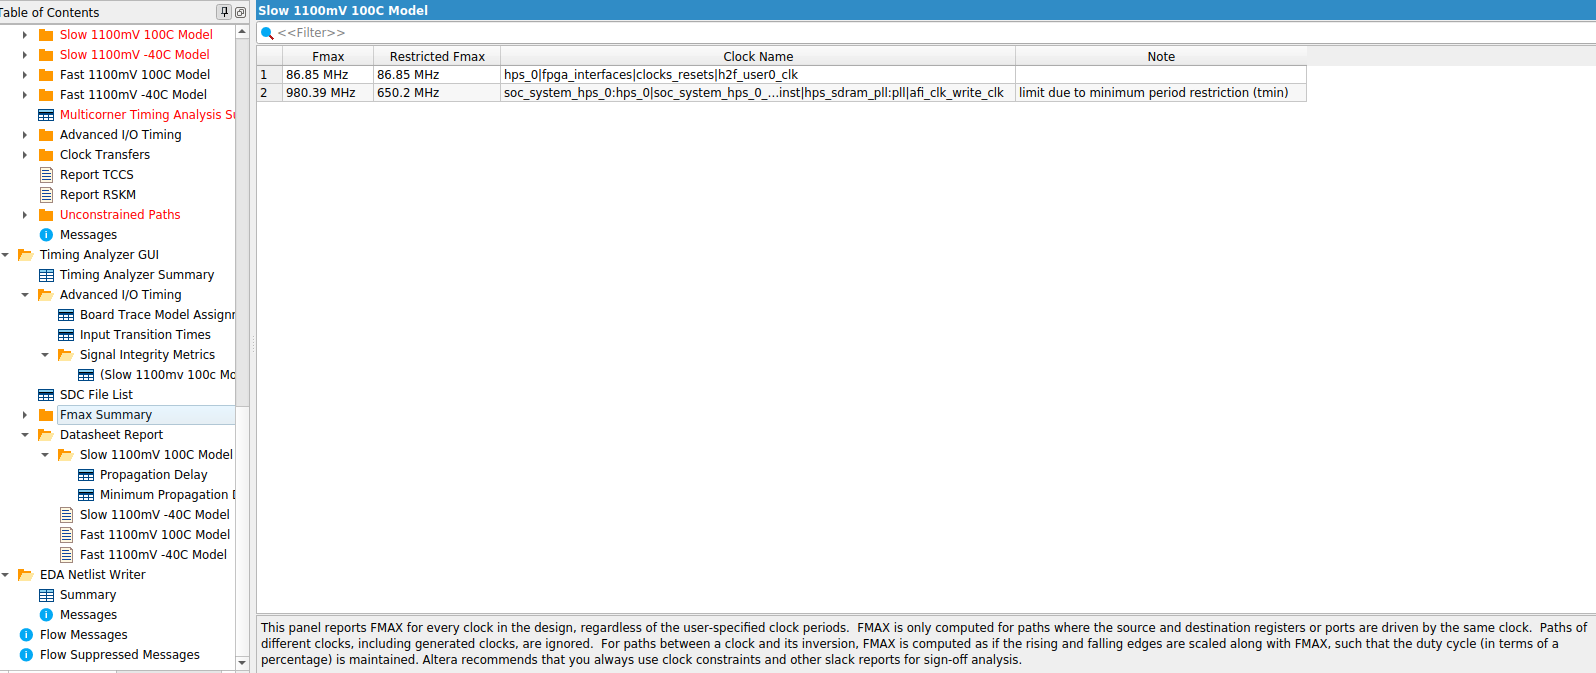
\includegraphics[width=\linewidth,height=0.27\textheight,keepaspectratio]{ffmax.png}
  \caption{Fmax Summary; clock \texttt{h2f\_user0\_clk} tercatat sebesar 86,85~MHz pada kompilasi ini.}
\end{figure}

\begin{figure}[H]
  \centering
  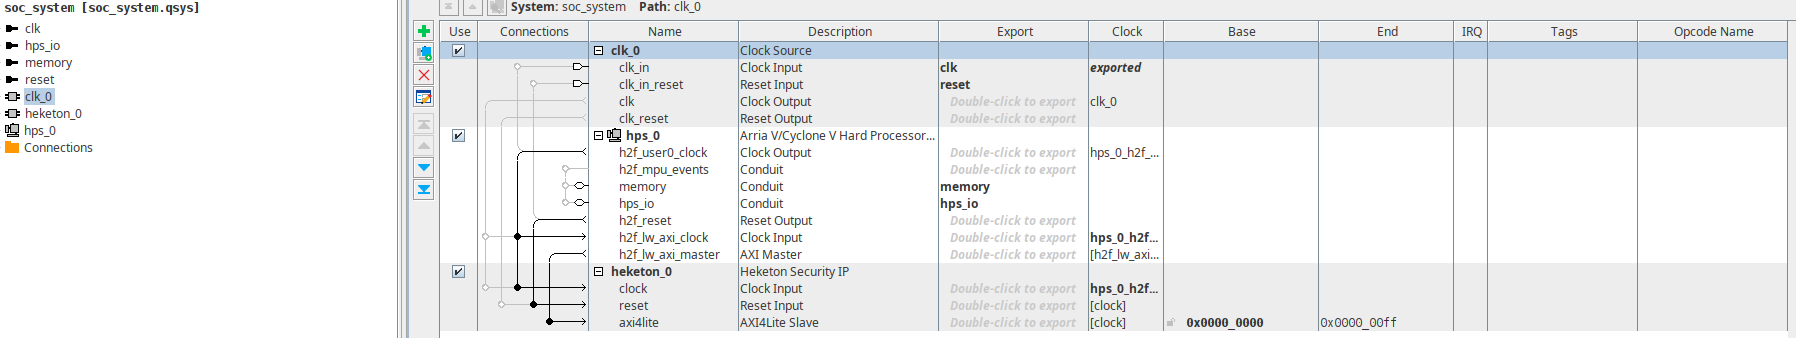
\includegraphics[width=\linewidth,height=0.27\textheight,keepaspectratio]{platformdesign.png}
  \caption{Platform Designer: HPS, lightweight AXI, dan HEKETON dalam sistem Qsys.}
\end{figure}

\section*{Tim \& Pembagian Peran}

\begin{center}
\small
\begin{tabularx}{\linewidth}{|>{\raggedright\arraybackslash}p{4.0cm}|>{\raggedright\arraybackslash}p{3.0cm}|X|}
\hline
\hdr{Nama} & \hdr{Peran} & \hdr{Tanggung jawab} \\ \hline
Guntur Sulistyo\newline{\footnotesize\color{subtle}Ketua} & Keamanan dan koordinasi & Model ancaman, desain \texttt{tamper\_mon}, uji serangan (\emph{replay}, \emph{glitch} clock, pembukaan casing), karakterisasi PUF, dan koordinasi tim. \\ \hline
Muhammad Muqtada Alhaddad & Perancang RTL & Seluruh modul RTL (\texttt{bus\_if}, \texttt{auth\_ctrl}, \texttt{ro\_puf}, \texttt{fuzzy\_ext}, \texttt{key\_vault}, \texttt{hmac\_sha256}), sintesis, \emph{timing closure}, dan porting ke DE10-Nano. \\ \hline
Dimas Eryan Ahnaf Fahrezi & Sistem dan verifikasi & Model referensi Python, \emph{testbench} C++/Verilator, emulasi stasiun dan basis data identitas, protokol enrolment, serta dokumentasi dan presentasi. \\ \hline
Ir. Agus Bejo, S.T., M.Eng., D.Eng., IPM & Dosen pembimbing & Arahan teknis dan tinjauan desain. \\ \hline
\end{tabularx}
\end{center}

\section*{Luaran \& Demo}

Luaran berikut direncanakan untuk tahap bootcamp dan final. Verifikasi RTL awal telah berjalan; demonstrasi dan karakterisasi pada DE10-Nano masih direncanakan.

\field{Demo Live:}
Demo direncanakan berjalan di DE10-Nano dengan dua ``baterai'' (dua lokasi PUF berbeda), dua stasiun emulasi, dan satu basis data identitas. Empat skenario akan ditunjukkan.
\begin{itemize}
  \item Baterai asli diterima di kedua stasiun.
  \item Baterai kloning ditolak.
  \item Respons lama yang dikirim ulang (\emph{replay}) ditolak.
  \item \emph{Glitch} clock atau pembukaan ``casing'' membuat chip terkunci dengan indikator LED, lalu ID-nya diblokir basis data.
\end{itemize}

\field{Video Demo:}
Video 3--5 menit akan berisi masalah baterai palsu, cara kerja chip bersama stasiun dan basis data, serta keempat skenario demo. Video ini juga disiapkan sebagai cadangan bila board bermasalah saat demo langsung.

\field{Repository Source Code:}
Repositori akan memuat RTL SystemVerilog, \emph{testbench} C++/Verilator, model referensi Python, emulasi stasiun dan basis data, proyek Quartus, skrip karakterisasi PUF, dan \emph{bitstream}.

\field{Laporan Teknis Singkat:}
Laporan akan memuat hasil pengukuran terhadap target R1--R5, yaitu statistik PUF (keunikan dan reliabilitas), latensi autentikasi, hasil sintesis (sumber daya, \emph{timing}, dan daya), serta hasil uji serangan. Laporan juga dilengkapi spesifikasi arsitektur dan \emph{register map}.

\section*{Rencana Bootcamp (3 Hari)}

\field{Jadwal \& Target Eksekusi:} RTL akan diuji lebih dulu pada FPGA milik tim sebelum bootcamp (Bagian~4.3). Bootcamp digunakan untuk memindahkan desain ke DE10-Nano dan mengukur target R1--R5. Jalur kritis dengan kunci tetap dikerjakan lebih dulu sehingga demo selalu dapat berjalan.

\begin{center}
\small
\renewcommand{\arraystretch}{1.15}
\begin{tabularx}{\linewidth}{|>{\centering\arraybackslash}p{1.4cm}|>{\raggedright\arraybackslash}p{4.0cm}|X|}
\hline
\hdr{Hari} & \hdr{Fokus Kegiatan} & \hdr{Target Deliverables} \\ \hline
\textbf{Hari 1} & Pindah ke DE10-Nano dengan kunci tetap & HMAC lolos vektor uji di board. Emulasi stasiun dan basis data di HPS dapat menerima atau menolak baterai. Uji \emph{replay} (R2). \\ \hline
\textbf{Hari 2} & Kunci dari PUF & \texttt{ro\_puf} dan \texttt{fuzzy\_ext} menggantikan kunci tetap. Keunikan dan reliabilitas PUF (R1), sumber daya, dan \emph{timing} (R5) terukur. \\ \hline
\textbf{Hari 3} & Uji serangan dan finalisasi & \emph{Glitch} clock dan pembukaan casing memicu hapus kunci dan \emph{lock} (R4). Skenario riwayat dan pemblokiran ID (R3). Video demo, laporan teknis, dan slide siap. \\ \hline
\end{tabularx}
\end{center}

\end{document}
